\begin{frame}
  \frametitle{Task description}
  \begin{columns}
    \begin{column}{0.45\textwidth}
      \centering
      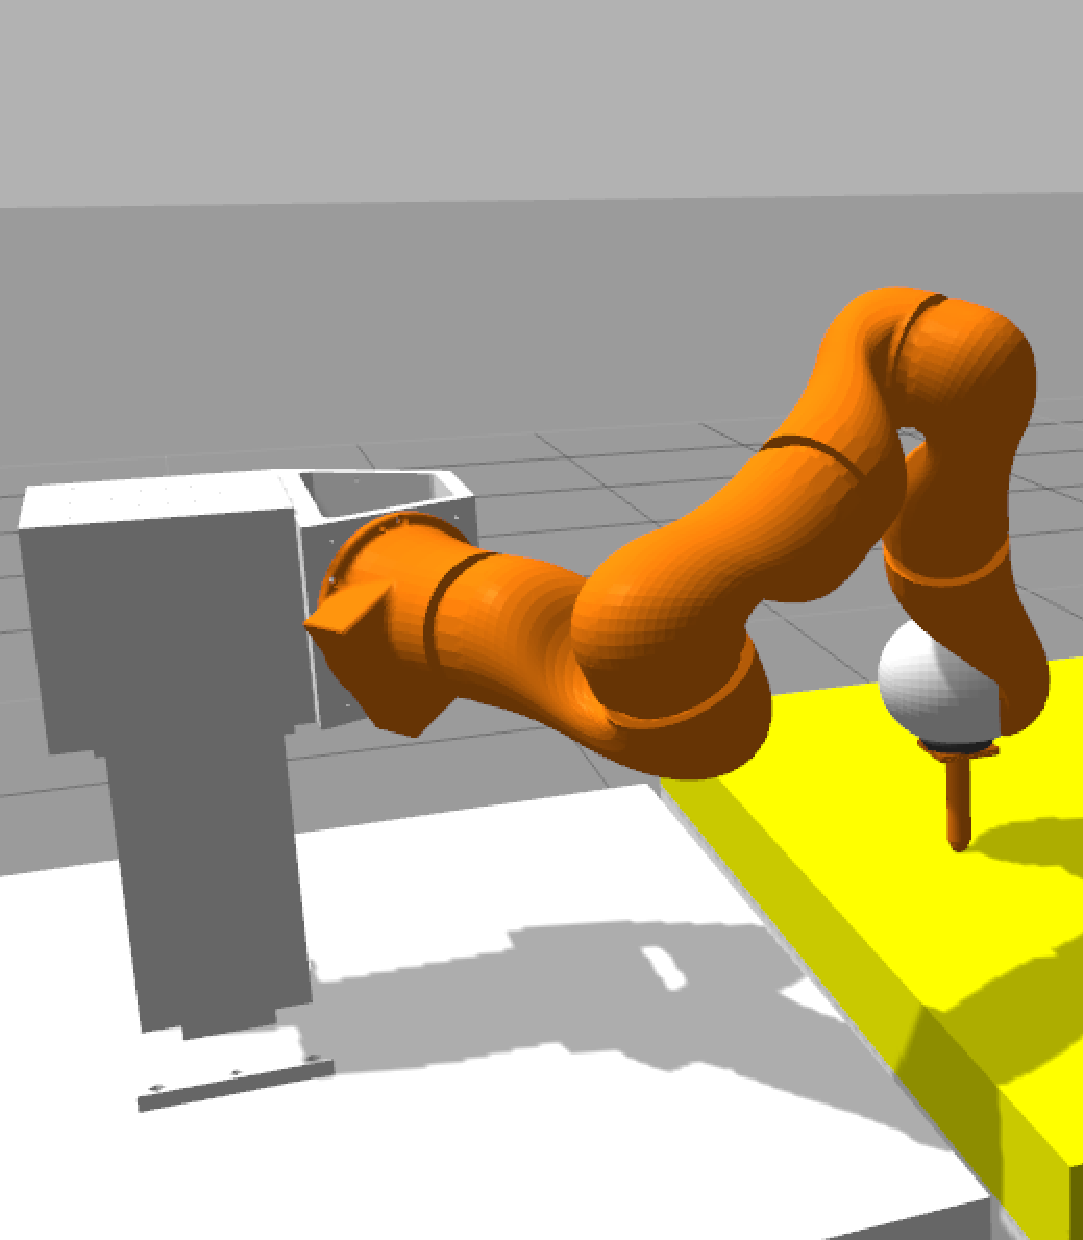
\includegraphics[width=\columnwidth]{task_picture}
    \end{column}
    \begin{column}{0.5\textwidth}
      Control objectives:
      \begin{itemize}
      \item[-] to command a trajectory on the surface of the table
      \item[-] to exert a force along the normal to the surface of the table
      \item[-] to be compliant on the surface of the table
      \end{itemize}
    \end{column}
  \end{columns}
\end{frame}
